\iffalse
A single-board computer Ż.Ŵ Image processing configurations
TODO: TABELL MED OVERSIKT OVER CONFIGS
Table 8.1: Image processing configurations
Hardware Computer Vision
Software
Weight
Config 1 Nvidia Jetson
Nano, ArduCamŻ.Ŵ Image processing configurations
TODO: TABELL MED OVERSIKT OVER CONFIGS
Table 8.1: Image processing configurations
Hardware Computer Vision
Software
Weight
Config 1 Nvidia Jetson
Nano, ArduCam
Mini
TensorRT,
YOLOv5
...
Config 2 Raspberry Pi 4,
Coral Edge TPU,
Pi Camera 3.0
OpenCV, Tensor-
Flow Lite
...
Config 3 Raspberry Pi Zero
Mini
TensorRT,
YOLOv8
...
Config 2 Raspberry Pi 4,
Coral Edge TPU,
Pi Camera 3.0
OpenCV, Tensor-
Flow Lite
...
Config 3 Raspberry Pi Zero 
\fi

\title{Hardware}
\section{Specification tables for configs}

All values from these tables that are not referenced externally are done by own measuring.\\
The power supply component for the single-board computers has been omitted from these tables due to there being several different options to choose from when supplying power to these boards and not all of them can be covered here.

\subsection{Config 1}

\begin{table}[!htb]
\begin{tabular}{ | >{\raggedright}p{\dimexpr 0.30\linewidth-2\tabcolsep} |
                   >{\raggedleft}p{\dimexpr 0.14\linewidth-2\tabcolsep} |
                   >{\raggedleft}p{\dimexpr 0.14\linewidth-2\tabcolsep} |
                   >{\raggedleft}p{\dimexpr 0.14\linewidth-2\tabcolsep} |
                    >{\raggedleft}p{\dimexpr 0.14\linewidth-2\tabcolsep} |
                   >{\raggedleft\arraybackslash}p{\dimexpr 0.14\linewidth-2\tabcolsep} | } \hline

&\bfseries{MSRP} & \bfseries{Weight} & \bfseries{Volume} & \bfseries{Power} (idle)   & \bfseries{Power (max)}    \\\hline

\bfseries{Jetson Nano}      & \$ 99     & 241 g     & 232 cm$^{3}$  & 5 W       & 10 W      \\\hline
\bfseries{Pi camera 3}      & \$ 25     & 4 g       & 7 cm$^{3}$    & 0,66 W    & 0,83 W    \\\hline
\bfseries{Camera ribbon}    & -         & 1,1 g     & -             & -         & -         \\\hline
\bfseries{SUM}              & \$ 124    & \bfseries{246,1 g}   & \bfseries{239 cm$^{3}$}    & \bfseries{5,7 W}    & \bfseries{10,8 W}    \\\hline
\end{tabular}
\caption{Hardware specification table for Config 1 hardware \cite{Jetson}\cite{specifications-cameras}}
\label{tab:spec_table_Config1}
\end{table}


\subsection{Config 2}

\begin{table}[!htb]
\begin{tabular}{ | >{\raggedright}p{\dimexpr 0.30\linewidth-2\tabcolsep} |
                   >{\raggedleft}p{\dimexpr 0.14\linewidth-2\tabcolsep} |
                   >{\raggedleft}p{\dimexpr 0.14\linewidth-2\tabcolsep} |
                   >{\raggedleft}p{\dimexpr 0.14\linewidth-2\tabcolsep} |
                    >{\raggedleft}p{\dimexpr 0.14\linewidth-2\tabcolsep} |
                   >{\raggedleft\arraybackslash}p{\dimexpr 0.14\linewidth-2\tabcolsep} | } \hline

&\bfseries{MSRP} & \bfseries{Weight} & \bfseries{Volume} & \bfseries{Power} (idle)   & \bfseries{Power (max)}    \\\hline

\bfseries{Raspberry Pi 4B 4GB}  & \$ 60     & 46 g      & 86 cm$^{3}$   & 2,7 W     & 6,4 W     \\\hline
\bfseries{Pi camera 3}          & \$ 25     & 4 g       & 7 cm$^{3}$    & 0,66 W    & 0,83 W    \\\hline
\bfseries{Camera ribbon}        & -         & 1,1 g     & -             & -         & -         \\\hline
\bfseries{Coral USB}            & \$ 60     & 19,7 g    & 15,6 cm$^{3}$ & 2,5 W     & 4,5 W     \\\hline
\bfseries{USB C-A cable}        & -         & 16,8 g    & -             & -         & -         \\\hline
\bfseries{SUM}                  & \$ 145 & \bfseries{87,6 g}   & \bfseries{109 cm$^{3}$}    & \bfseries{5,7 W}    & \bfseries{11,7 W}    \\\hline
\end{tabular}
\caption{Hardware specification table for Config 2 hardware \cite{datasheet-RPi4B}\cite{power-consumption-RPi4}\cite{specifications-cameras}\cite{CoralTPU}}
\label{tab:spec_table_Config2}
\end{table}

\newpage

\subsection{Config 3}

\begin{table}[!htb]
\begin{tabular}{ | >{\raggedright}p{\dimexpr 0.30\linewidth-2\tabcolsep} |
                   >{\raggedleft}p{\dimexpr 0.14\linewidth-2\tabcolsep} |
                   >{\raggedleft}p{\dimexpr 0.14\linewidth-2\tabcolsep} |
                   >{\raggedleft}p{\dimexpr 0.14\linewidth-2\tabcolsep} |
                    >{\raggedleft}p{\dimexpr 0.14\linewidth-2\tabcolsep} |
                   >{\raggedleft\arraybackslash}p{\dimexpr 0.14\linewidth-2\tabcolsep} | } \hline

&\bfseries{MSRP} & \bfseries{Weight} & \bfseries{Volume} & \bfseries{Power} (idle)   & \bfseries{Power (max)}    \\\hline

\bfseries{Raspberry Pi Zero2}   & \$ 15     & 11 g      & 9,75 cm$^{3}$     & 0,6 W     & 6,4 W     \\\hline
\bfseries{Pi camera 3}          & \$ 25     & 4 g       & 7 cm$^{3}$        & 0,66 W    & 0,83 W    \\\hline
\bfseries{Camera ribbon}        & -         & 1,1 g     & -                 & -         & -         \\\hline
\bfseries{Coral USB}            & \$ 60     & 19,7 g    & 15,6 cm$^{3}$     & 2,5 W     & 4,5 W     \\\hline
\bfseries{USB C-micro cable}    & -         & 7,5 g     & -                 & -         & -         \\\hline
\bfseries{SUM}                  & \$ 100 & \bfseries{43,3 g}   & \bfseries{32 cm$^{3}$}    & \bfseries{3,8 W}    & \bfseries{11,7 W}    \\\hline
\end{tabular}
\caption{Hardware specification table for Config 3 hardware \cite{datasheet-RPiZero2}\cite{power-consumption-RPiZero2}\cite{specifications-cameras}\cite{CoralTPU}}
\label{tab:spec_table_Config3}
\end{table}



\subsection{Config 4}

\begin{table}[!htb]
\begin{tabular}{ | >{\raggedright}p{\dimexpr 0.30\linewidth-2\tabcolsep} |
                   >{\raggedleft}p{\dimexpr 0.14\linewidth-2\tabcolsep} |
                   >{\raggedleft}p{\dimexpr 0.14\linewidth-2\tabcolsep} |
                   >{\raggedleft}p{\dimexpr 0.14\linewidth-2\tabcolsep} |
                    >{\raggedleft}p{\dimexpr 0.14\linewidth-2\tabcolsep} |
                   >{\raggedleft\arraybackslash}p{\dimexpr 0.14\linewidth-2\tabcolsep} | } \hline

&\bfseries{MSRP} & \bfseries{Weight} & \bfseries{Volume} & \bfseries{Power} (idle)   & \bfseries{Power (max)}    \\\hline

\bfseries{Raspberry Pi 4B}  & \$ 60     & 46 g      & 86 cm$^{3}$   & 2,7 W     & 6,4 W     \\\hline
\bfseries{Pi camera 3}      & \$ 25     & 4 g       & 7 cm$^{3}$    & 0,66 W    & 0,83 W    \\\hline
\bfseries{Camera ribbon}    & -         & 1,1 g     & -             & -         & -         \\\hline
\bfseries{SUM}              & \$ 85 & \bfseries{51,1 g} & \bfseries{93 cm$^{3}$}  & \bfseries{3,4 W}  & \bfseries{7,2 W}    \\\hline

\end{tabular}
\caption{Hardware specification table for Config 4 hardware \cite{datasheet-RPi4B}\cite{power-consumption-RPi4}\cite{specifications-cameras}}
\label{tab:spec_table_Config4}
\end{table}

\subsection{Comparison}

\begin{table}[!htb]
\begin{tabular}{ | >{\raggedright}p{\dimexpr 0.30\linewidth-2\tabcolsep} |
                   >{\raggedleft}p{\dimexpr 0.14\linewidth-2\tabcolsep} |
                   >{\raggedleft}p{\dimexpr 0.14\linewidth-2\tabcolsep} |
                   >{\raggedleft}p{\dimexpr 0.14\linewidth-2\tabcolsep} |
                    >{\raggedleft}p{\dimexpr 0.14\linewidth-2\tabcolsep} |
                   >{\raggedleft\arraybackslash}p{\dimexpr 0.14\linewidth-2\tabcolsep} | } \hline

&\bfseries{MSRP} & \bfseries{Weight} & \bfseries{Volume} & \bfseries{Power} (idle)   & \bfseries{Power (max)}    \\\hline

\bfseries{Config 1}& \$ 124     & 246,1 g   & 239 cm$^{3}$  & 5,7 W     & 10,8 W    \\\hline
\bfseries{Config 2}& \$ 145     & 87,6 g    & 109 cm$^{3}$  & 5,7 W     & 11,7 W    \\\hline
\bfseries{Config 3}& \$ 100    & 43,3 g    & 32 cm$^{3}$   & 3,8 W     & 11,7 W    \\\hline
\bfseries{Config 4}& \$ 85    & 51,1 g    & 93 cm$^{3}$   & 3,4 W     & 7,2 W     \\\hline

\end{tabular}
\caption{Hardware specification table for comparison of all configs}
\label{tab:spec_table_comparison}
\end{table}

\section{Single-board computer (SBC)}

A single-board computer (SBC) is a complete computer built on a single circuit board, with microprocessor(s), memory, input/output (I/O) and other features required of a functional computer. Single-board computers are commonly made as demonstration or development systems, for educational systems, or for use as embedded computer controllers. Many types of home computers or portable computers integrate all their functions onto a single printed circuit board.

Unlike a desktop personal computer, single board computers often do not rely on expansion slots for peripheral functions or expansion. Single board computers have been built using a wide range of microprocessors. Simple designs, such as those built by computer hobbyists, often use static RAM and low-cost 32- or 64-bit processors like ARM. Other types, such as blade servers, would perform similar to a server computer, only in a more compact format. \cite{SBC}

Thanks to the characteristics of SBCs, they are a core hardware component in all of the architectural designs in this comparative study.

\newpage
\begin{table}
\begin{tabular}{ | >{\raggedright}p{\dimexpr 0.19\linewidth-2\tabcolsep} |
                   >{\raggedleft}p{\dimexpr 0.27\linewidth-2\tabcolsep} |
                   >{\raggedleft}p{\dimexpr 0.27\linewidth-2\tabcolsep} |
                   >{\raggedleft\arraybackslash}p{\dimexpr 0.27\linewidth-2\tabcolsep} | } \hline

                            & \centering\bfseries{RPi 4B} & \centering\bfseries{RPi Zero2} & \centering\arraybackslash\bfseries{Jetson Nano}\\\hline
\bfseries{CPU}              & Cortex-A72 @ 1.5GHz       & Cortex-A53 @ 1.0GHz   & Cortex-A57 @ 1.43GHz \\\hline
\bfseries{GPU}              & VideoCore IV @ 500MHz     & VideoCore IV @ 400MHz & 128-core Maxwell @ 921MHz \\\hline
\bfseries{Memory}           & 1 GB - 8 GB               & 512 MB                & 4 GB \\\hline
\bfseries{Video decoding}   & H.264/H.265 (4Kp60)       & H.264 (1080p30)       & H.264/H.265 (4Kp60) \\\hline
\bfseries{Video encoding}   & H.264/H.265 (1080p30)     & H.264 (1080p30)       & H.264/H.265 (4Kp30) \\\hline
\bfseries{Connectivity}     & USB 3.0 × 2               & USB 2.0 × 1           & USB 3.0 × 4 \\
                            & USB 2.0 × 2               & UART × 1              & USB 2.0 × 1 \\
                            & UART × 1                  & SPI × 2               & UART × 1 \\
                            & SPI × 2                   & I2C × 1               & SPI × 2 \\
                            & I2C × 1                   &                       & I2C × 3 \\\hline
\bfseries{Form factor}      & 85mm × 56mm               & 65mm × 30mm           & 69mm × 45mm \\\hline
\bfseries{Weight}           & 46g                       & 11g                   & 250g \\\hline
\bfseries{MSRP}             & \$ 35 - \$ 75             & \$ 15                 & \$ 99 \\\hline

\end{tabular}
\caption{Comparison table for single-board computers (SBCs) \protect\cite{datasheet-RPiZero2}\cite{datasheet-RPi4B}\cite{datasheet-JetsonNano}}
\label{tab:comparison_table_SBCs}
\end{table}

When proposing what SBCs to deploy in our test-solution architectures we tend to mainly look at specifications regarding processing power (CPU \& GPU), memory (RAM), hardware-accelerated video encoding/decoding and connectivity (USB, UART etc.) in relation to the weight and form factor of the board. We also need to take into consideration the availability and discrepancy between MSRP and actual sale price due to the current world-wide chip shortage disrupting the market.\\

We decided the top-contenders and implemented them across all configurations:
\begin{itemize}
    \item Raspberry Pi Zero 2 (RPi Zero 2)
    \item Raspberry Pi 4B (RPi 4B)
    \item nVidia Jetson Nano
\end{itemize}

% Fjerne denne? Usikker:
\iffalse
\subsection{nVidia Jetson Nano}
Jetson Nano Developer Kit is a compact, high-performance computer designed to run multiple neural networks simultaneously for applications such as image classification, object detection, segmentation, and speech processing. It enables developers to build AI-powered applications and projects using GPU acceleration. The Jetson Nano comes with a quad-core ARM CPU, NVIDIA GPU with 128 CUDA cores, and 4GB of RAM, making it suitable for applications like robotics, computer vision, and edge computing.\cite{Jetson}

\begin{figure}[h]
    \centering
    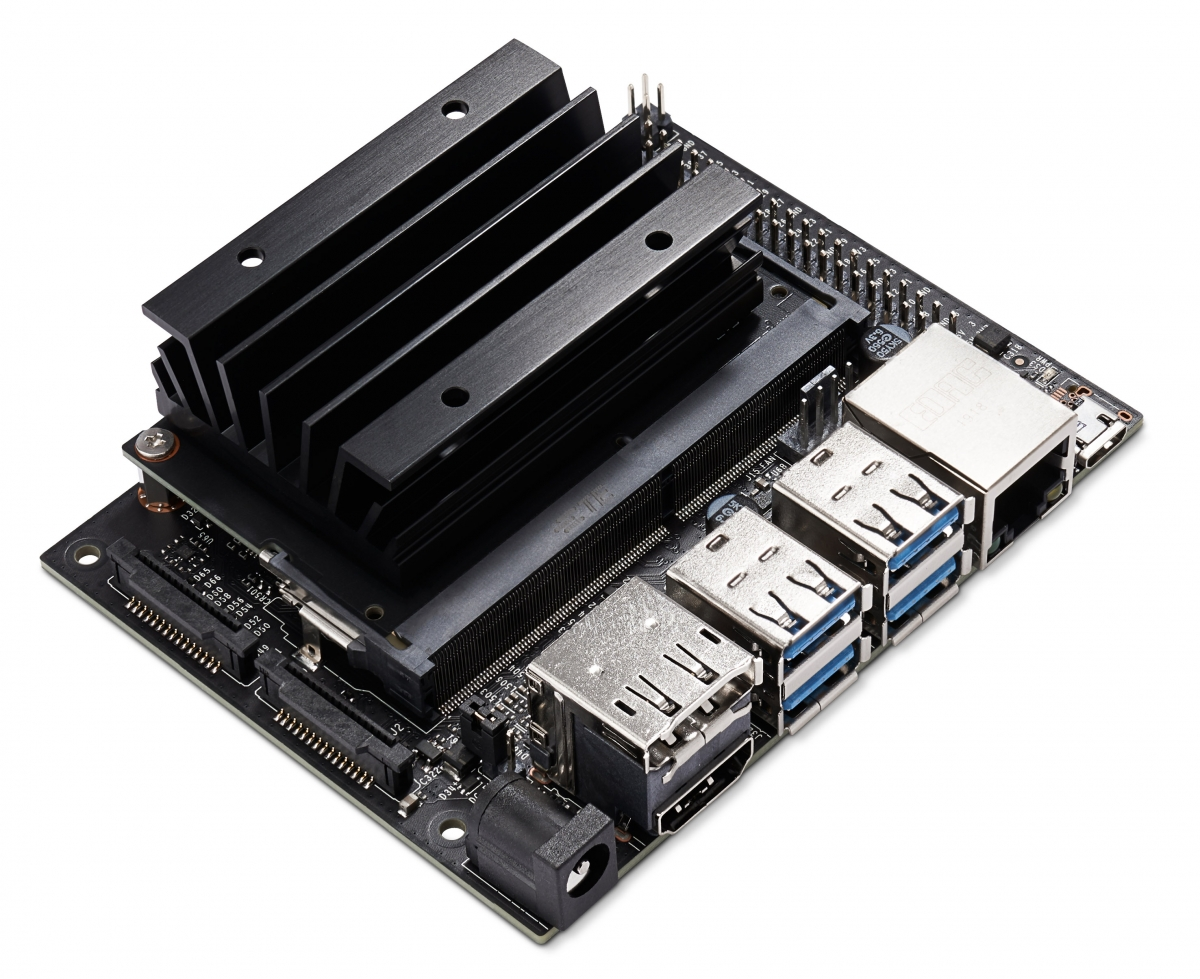
\includegraphics[scale=0.3]{fig/JetsonNano-DevKit_Front-Top_Right_trimmed.jpg}
    \caption{Jetson nano \cite{Jetson}}
\end{figure}
\fi


\newpage

\section{Camera}

\begin{table}[!h]
\begin{tabular}{ | >{\raggedright}p{\dimexpr 0.25\linewidth-2\tabcolsep} |
                   >{\raggedleft}p{\dimexpr 0.25\linewidth-2\tabcolsep} |
                   >{\raggedleft}p{\dimexpr 0.25\linewidth-2\tabcolsep} | 
                   >{\raggedleft\arraybackslash}p{\dimexpr 0.25\linewidth-2\tabcolsep} | } \hline

& \centering\bfseries{Camera Module v2}   & \centering\bfseries{Camera Module 3 NoIR}   & \centering\arraybackslash\bfseries{Camera Module 3 Wide} \\\hline
\bfseries{Video Modes}
& 1920 × 1080p47                & 2304 × 1296p56                    & 2304 × 1296p56 \\
& 1640 × 1232p41                & 2304 × 1296p30                    & 2304 × 1296p30 \\
& 640 × 480p206                 & 1536 × 864p120                    & 1536 × 864p120 \\\hline
\bfseries{Focus}
& Adjustable                    & Motorized                         & Motorized  \\\hline
\bfseries{Depth of field}
& Approx 10 cm to ∞             & Approx 10 cm to ∞                 & Approx 5 cm to ∞ \\\hline
\bfseries{Horizontal FoV}
& 62.2 degrees                  & 66 degrees                        & 102 degrees \\\hline
\bfseries{Vertical FoV}
& 48.8 degrees                  & 41 degrees                        & 67 degrees \\\hline
\bfseries{Size}
& 25 × 24 × 9mm                 & 25 × 24 × 11.5mm                  & 25 × 24 × 12.4mm \\\hline
\bfseries{Weight}
& 3g                            & 4g                                & 4g \\\hline
\bfseries{MSRP}
& \$ 25                         & \$ 25                             & \$ 35\\\hline
\end{tabular}
\caption{Comparison table for selected cameras\cite{specifications-cameras}}
\end{table}

\subsection{Rolling vs. Global shutter}
All the cameras selected for this project use a "rolling shutter", meaning each frame of a video is captured not by taking a snapshot of the entire scene at a single instant in time but rather by scanning across the scene rapidly, vertically, horizontally or rotationally. In other words, not all parts of the image of the scene are recorded at exactly the same instant. (Though, during playback, the entire image of the scene is displayed at once, as if it represents a single instant in time.) This produces predictable distortions of fast-moving objects or rapid flashes of light. This is in contrast with "global shutter" in which the entire frame is captured at the same instant. \cite{wikipedia-rolling-shutter}\\
A camera using a "global shutter" would therefore cause less distortion of objects in frame moving very fast, for example in the case of a drone capturing high-speed video footage.

\subsubsection{Raspberry Pi Global Shutter Camera}
Raspberry Pi recently released a new camera during this spring named the "Global Shutter (GS) Camera". The Global Shutter Camera’s image sensor has a 6.3mm diagonal active sensing area, which is similar in size to Raspberry Pi’s HQ Camera. However, the pixels are larger and can collect more light. Large pixel size and low pixel count are valuable in machine-vision applications; the more pixels a sensor produces, the harder it is to process the image in real time. To get around this, many applications downsize and crop images. This is unnecessary with the Global Shutter Camera and the appropriate lens magnification, where the lower resolution and large pixel size mean an image can be captured natively. \cite{documentation-RPi_cameras}\\
The new "GS Camera" would likely work substantially better for the application of capturing video on a drone for object detection, with the only drawback being additional weight from a heavier lens.

\iffalse
\subsection{Pi Camera module v2}
The Raspberry Pi Camera Module v2 was introduced in April 2016 to replace the original Camera Module. The v2 Camera Module is equipped with a Sony IMX219 8-megapixel sensor, which represents a significant upgrade from the 5-megapixel OmniVision OV5647 sensor found in the original camera. The Camera Module is capable of capturing high-definition video and still photographs. It is user-friendly for beginners, but also offers advanced features for users seeking to expand their knowledge. Online examples showcase the camera's versatility for time-lapse, slow-motion, and other video applications, while libraries provided with the camera facilitate the creation of special effects.\\

Further details about the IMX219 and the Exmor R back-illuminated sensor architecture are available on Sony's website, underscoring that the camera's improved resolution represents a leap forward in image quality, color fidelity, and low-light performance. The Camera Module supports 1080p30, 720p60, and VGA90 video modes, in addition to still capture. It attaches via a 15cm ribbon cable to the Camera Serial Interface (CSI) port on the Raspberry Pi, and is compatible with all models of Raspberry Pi 1, 2, and 3. The camera can be accessed through the Multi-Media Abstraction Layer (MMAL) and Video for Linux (V4L) APIs, and numerous third-party libraries are available, such as the Picamera Python library. A "Getting Started with Picamera" resource is available for users seeking guidance on its use. The Camera Module is widely employed in home security applications, as well as in wildlife camera traps.\cite{rpicam2specs}\cite{rpicamspecs}\\


\subsection{Pi Camera module v3}
The Raspberry Pi Camera Module 3 is a compact camera designed by Raspberry Pi, equipped with a 12-megapixel sensor featuring high dynamic range (HDR) and phase detection autofocus. The camera is available in standard and wide-angle variants, both with or without an infrared cut filter.\\

Capable of capturing full HD video and still photographs, the Camera Module 3 includes an HDR mode for up to 3 megapixels. Its operation is fully supported by the libcamera library, and its rapid autofocus feature makes it accessible to beginners while providing ample functionality for advanced users. The Camera Module 3 is compatible with all Raspberry Pi computers and features the same printed circuit board (PCB) size and mounting holes as its predecessor, the Camera Module 2. The only difference in dimension is the height, with the improved optics making the Camera Module 3 several millimetres taller than its predecessor.\cite{rpicam3specs} \\
\fi

\subsection{Camera drivers}
There are currently two different driver libraries for capturing with the Raspberry Pi Cameras:
\begin{itemize}
  \item libcamera \cite{docs-libcamera}
  \item RaspiCam (legacy) \cite{github-raspicam}
\end{itemize}

Some quick benchmark tests indicates that the legacy RaspiCam drivers outperforms the newer libcamera drivers in terms of CPU-usage. The reason for this is likely that the legacy drivers are proprietorially made by the own producer of the Rasberry Pi's GPU-stack (Broadcom) and are therefore more efficiently taking advantage of the hardware.\\\\
Below are screenshots of an RTP-stream, the first using piped output from "libcamera-vid" and the second using "v4l2src", both with a Pi Camera Module v2.\\
The \%CPU usage is over double for the "libcamera-vid" command compared to "v4l2src" when streaming @ 1080p30.

\begin{figure}[!htb]
    \centering
    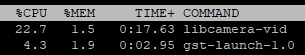
\includegraphics[width=\textwidth]{fig/gstreamer-libcamera_top_v2.png}
        \caption{libcamera-vid piping video to gstreamer}
\end{figure}

\begin{figure}[!htb]
    \centering
    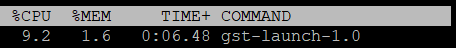
\includegraphics[width=\textwidth]{fig/gstreamer-raspicam_top_v2.png}
    \caption{v4l2src (RaspiCam) feeding video to gstreamer}
\end{figure}

Unfortunately, the newest Pi Camera Module v3 is not compatible with the legacy RaspiCam drivers.

\section{Hardware Acceleration for ML Inference}

\subsection{Google Coral TPU}
The Coral TPU is a compact, power-efficient chip designed by Google to accelerate TensorFlow Lite models on devices. It enables rapid machine learning processing, enhances data privacy, and eliminates the need for continuous internet connectivity. Developers can achieve high-performance machine learning inferencing, making it an ideal choice for applications like computer vision and natural language processing in various edge devices. \cite{CoralTPU}

\begin{figure}[h]
    \centering
    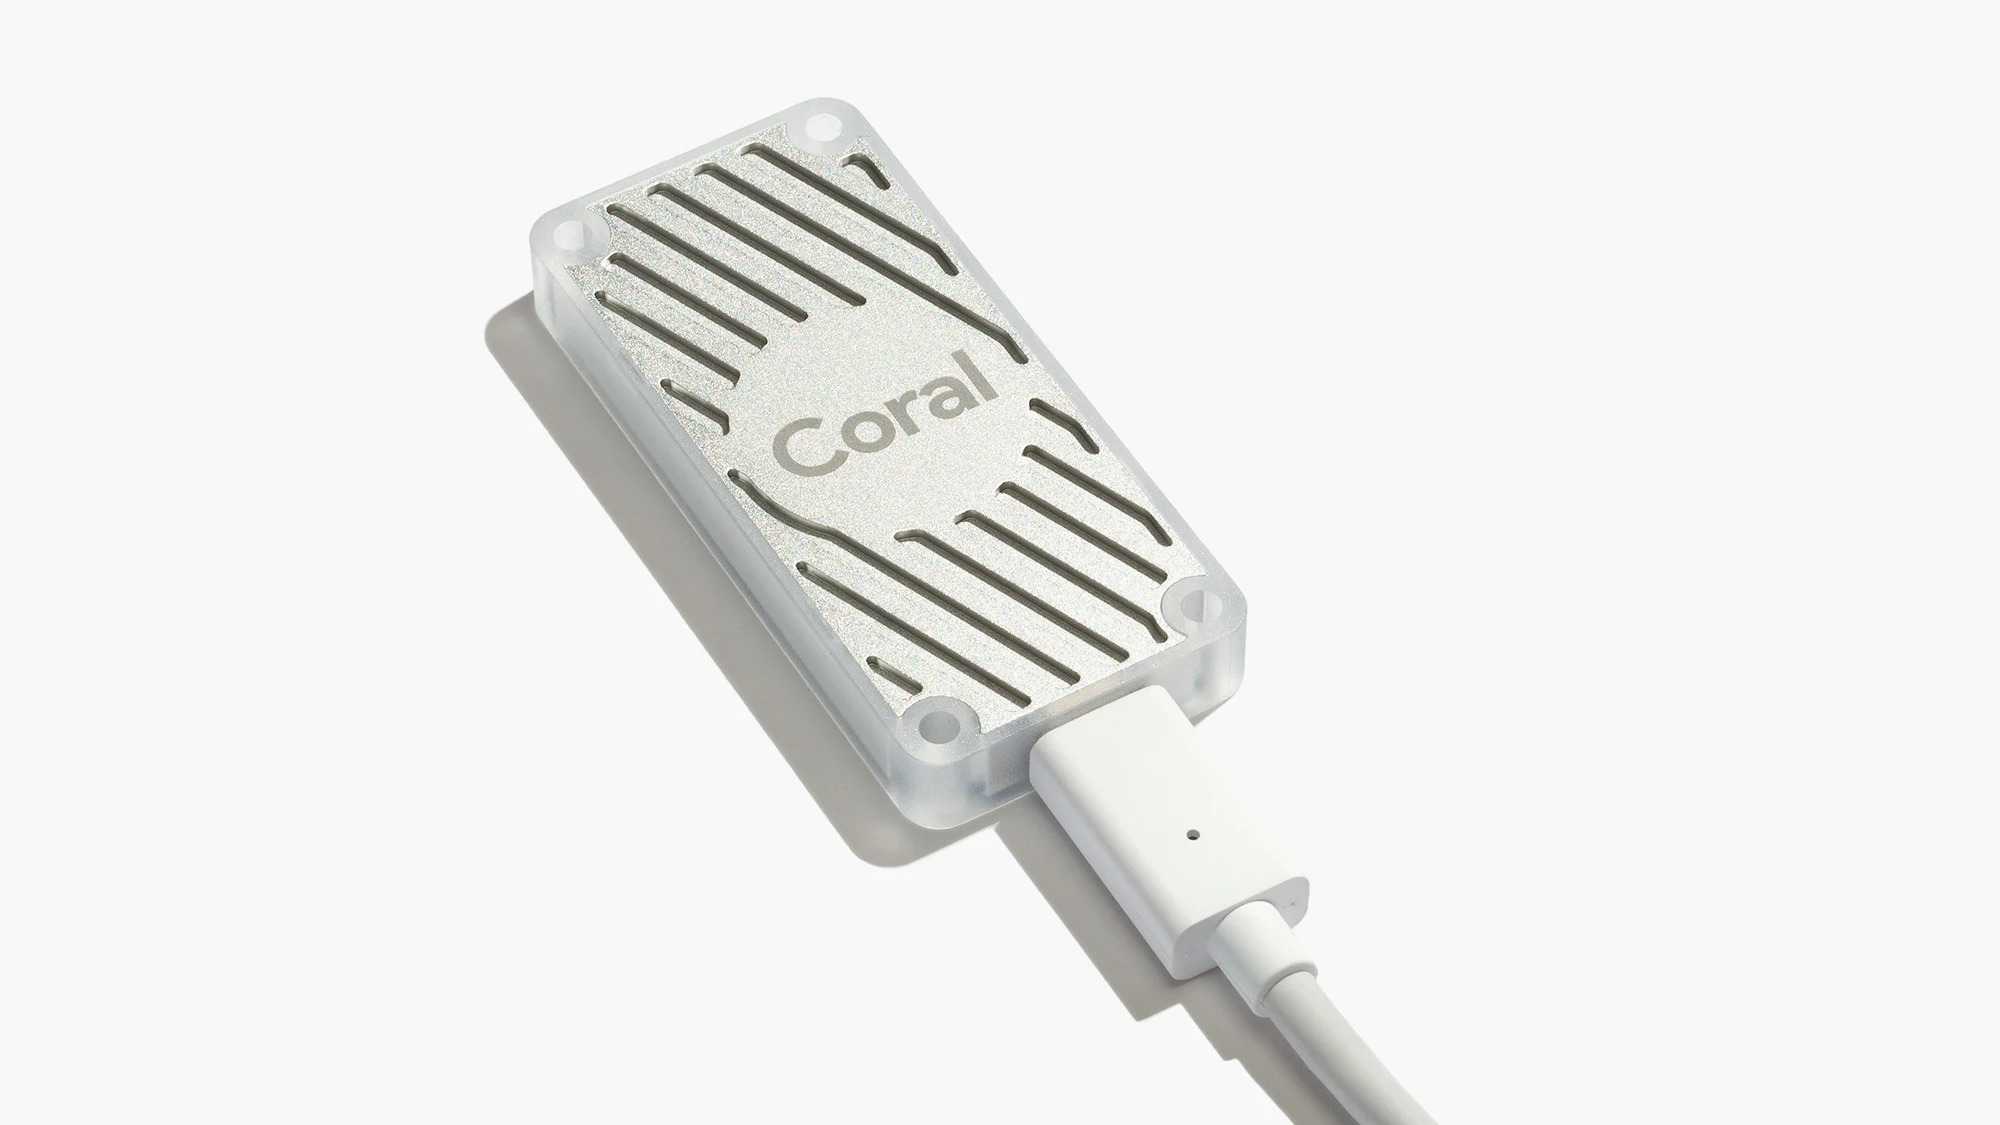
\includegraphics[scale=0.15]{fig/Coral TPU.jpg}
    \caption{Coral USB accelerator \cite{CoralTPU_bilde}}
\end{figure}

\section{Flight controller}
\label{fc}

When choosing flight controller (FC) board(s) for the hardware stack of our test-solution architectures we tend to mainly look at processor speed and flash memory in relation to form factor and weight as well as the availability in local retail shops. The boards' sensor and connectivity options are aspects we deem less relevant for our research project.

F1, F3, F4, G4, F7, and H7 are the different STM32 processors (aka MCU – Micro Controller Unit). The processor is the brain of a flight controller (FC), similar to the CPU in a computer.

There are currently 11 series of STM32 MCU, from faster to slower processing speeds they are: H7, F7, G4, F4, F3, F2, F1, F0, L4, L1, and L0. \cite{comparison-FC}

We decided to go for a single FC to be used in all the hardware stacks of our test-solution architectures of the latest and greatest generation FC that employs the fastest H7-generation microcontroller unit (MCU) with 2 MB of flash memory. This ensures the drone can run very smoothly and has sufficient flash memory to support any firmware with a full set of features.

\begin{table}
\begin{tabular}{ | >{\raggedright}p{\dimexpr 0.26\linewidth-2\tabcolsep} |
                   >{\raggedleft}p{\dimexpr 0.25\linewidth-2\tabcolsep} |
                   >{\raggedleft}p{\dimexpr 0.25\linewidth-2\tabcolsep} |
                   >{\raggedleft\arraybackslash}p{\dimexpr 0.24\linewidth-2\tabcolsep} | } \hline

\bfseries{Processor}        & \centering\bfseries{Processor Speed}    & \centering\bfseries{Flash Memory}   & \centering\arraybackslash\bfseries{SRAM} \\\hline
\bfseries{F0 (STM32F051)}   & 48MHz                         & 256KB                     & 32KB  \\\hline
\bfseries{F1 (STM32F103)}   & 72MHZ                         & 128KB                     & 96KB  \\\hline
\bfseries{F3 (STM32F303)}   & 72MHz                         & 256KB                     & 80KB  \\\hline
\bfseries{F4 (STM32F405)}   & 168MHz                        & 1MB                       & 192KB \\\hline
\bfseries{F4 (STM32F411)}   & 100MHz                        & 512KB                     & 128KB \\\hline
\bfseries{G4 (STM32G491)}   & 170MHz                        & 512KB                     & 128KB \\\hline
\bfseries{F7 (STM32F745)}   & 216MHz                        & 1MB                       & 320KB \\\hline
\bfseries{F7 (STM32F722)}   & 216MHz                        & 512KB                     & 256KB \\\hline
\bfseries{F7 (STM32F765)}   & 216MHz                        & 2MB                       & 512KB \\\hline
\bfseries{H7 (STM32H743)}   & 480MHz                        & 2MB                       & 1MB   \\\hline

\end{tabular}
\caption{Comparison table for microcontroller unit (MCU) \protect\cite{comparison-FC}}
\end{table}

We decided we wanted to go for a single FC for the hardware stacks of our test-solution architectures. Employing the "STM32H743" MCU, it ensures the drone can run very smoothly and has sufficient flash memory to support any firmware with a full set of features.

We ended up going for a MATEKSYS Flight Controller H743-SLIM \cite{MateksysH743-SLIM} as it fulfills our criteria and could be readily ordered at the Norwegian online store "elefun.no".

\begin{figure}[!htb]
    \centering
    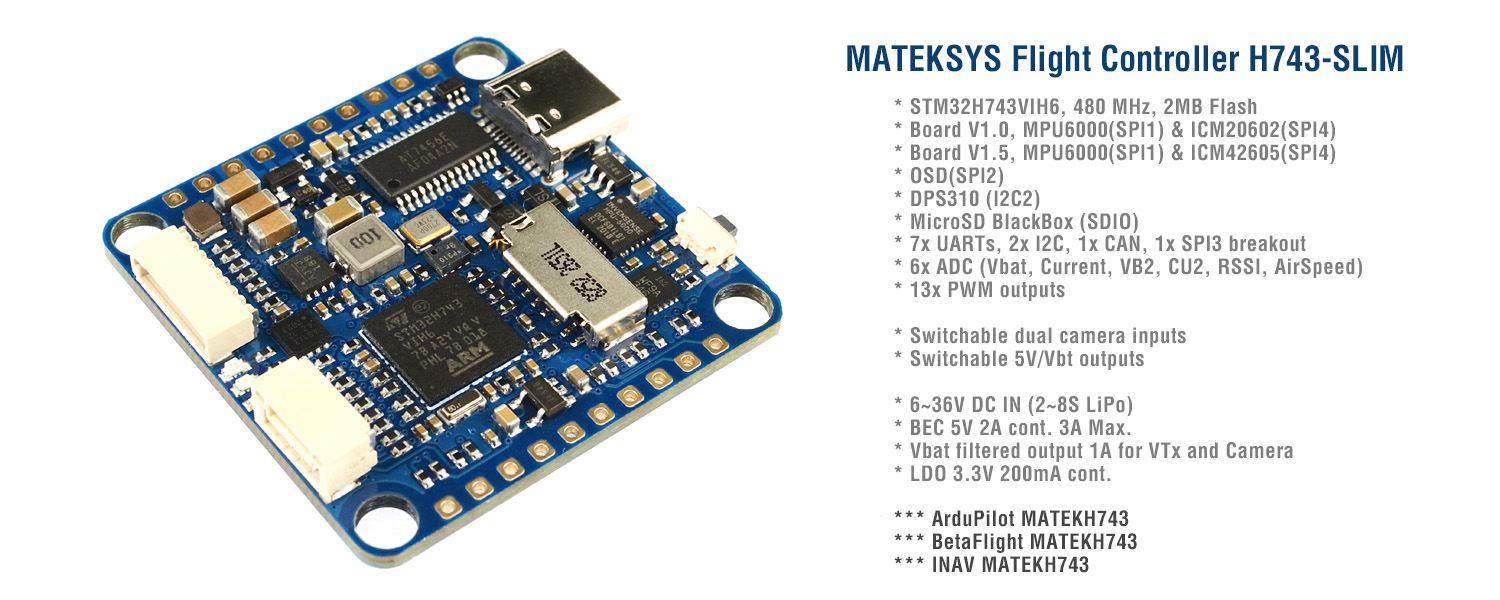
\includegraphics[width=\textwidth]{fig/H743-SLIM_1.jpg}
    \caption{Showcase of MATEKSYS H743-SLIM, from mateksys.com \protect\cite{MateksysH743-SLIM}}
\end{figure}

\newpage


% Deaktiverer denne:
\iffalse
\subsection{PID controller for autonomous flying}

A proportional–integral–derivative controller (PID controller or three-term controller) is a control loop mechanism employing feedback that is widely used in industrial control systems and a variety of other applications requiring continuously modulated control. A PID controller continuously calculates an error value e(t) as the difference between a desired setpoint (SP) and a measured process variable (PV) and applies a correction based on proportional, integral, and derivative terms (denoted P, I, and D respectively), hence the name. \cite{wiki-PID-controller}

\begin{figure}[!htb]
    \centering
    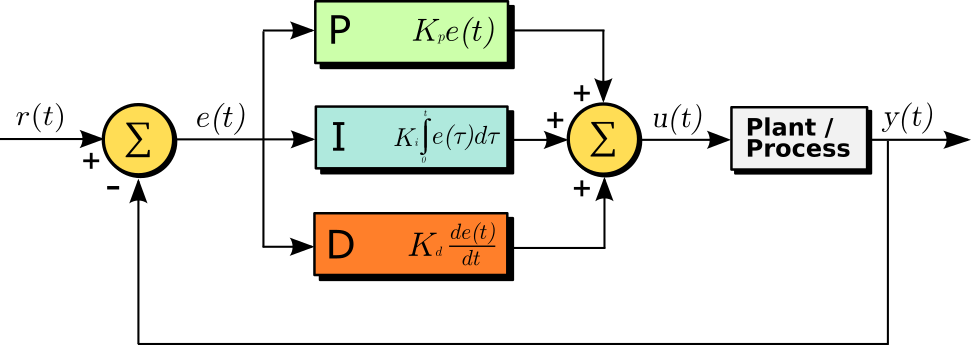
\includegraphics[width=\textwidth]{fig/PID-controller.png}
    \caption{PID controller, from wikipedia.org \protect\cite{wiki-PID-controller}}
\end{figure}

We believe in this stage of the project that it's possible to employ a PID controller program for real-time calculation of the drone's desired action while fed input data from an object detection program running in parallel.
The PID controller program will then generate MAVLink messages to somehow control the drone. This can possibly be done through MAVLink's Manual Control Protocol.
\fi